% This is samplepaper.tex, a sample chapter demonstrating the
% LLNCS macro package for Springer Computer Science proceedings;
% Version 2.21 of 2022/01/12
%
\documentclass[runningheads]{llncs}
\usepackage[T1]{fontenc}
\usepackage[hidelinks]{hyperref}
\usepackage{pgfplots}
\usepackage{float}
\usepackage[utf8]{inputenc}
\usepackage{hyperref}
\usepackage{booktabs}
\usepackage{tabularx}
\usepackage{booktabs}
\usepackage{tikz}
\usepackage{parskip}
\usetikzlibrary{shapes.geometric, arrows.meta, positioning}

% T1 fonts will be used to generate the final print and online PDFs,
% so please use T1 fonts in your manuscript whenever possible.
% Other font encondings may result in incorrect characters.

% --- AJUSTES DE ESPACIADO PARA EVITAR HUECOS BLANCOS ---
\setlength{\textfloatsep}{5pt}
\setlength{\floatsep}{5pt}

% Used for displaying a sample figure. If possible, figure files should
% be included in EPS format.
%
% If you use the hyperref package, please uncomment the following two lines
% to display URLs in blue roman font according to Springer's eBook style:
%\usepackage{color}
%\renewcommand\UrlFont{\color{blue}\rmfamily}
%\urlstyle{rm}
%
\raggedbottom
\begin{document}
%
\title{Experimental evaluation of georeferenced validation in a biometric attendance system under Wi-Fi, mobile data, and VPN networks}

\titlerunning{Georeferenced validation in a biometric system}

\author{Edith Liliana Chuico Navarrete\inst{1}\orcidID{0009-0008-6824-7647} \and
Geovanny José Brito Casanova\inst{2}\orcidID{0000-0002-7715-7706}}

\authorrunning{E. L. Chuico Navarrete et al.}

\institute{Universidad de las Fuerzas Armadas ESPE, Sangolquí, Ecuador \\
\email{\{elchuico, jgbrito\}@espe.edu.ec}\\
\url{www.espe.edu.ec}}

\maketitle               % typeset the header of the contribution
%
\begin{abstract}
Geofencing-based attendance systems often ignore how connectivity alters coordinate acquisition and validation performance. This study aims to evaluate the effect of Wi-Fi, mobile data, and VPN networks on accuracy, acquisition time, and decision-making in a distributed attendance architecture. A quantitative experimental methodology with a factorial design ($2\times2\times2$) was applied, analyzing 160 clock-ins across eight scenarios inside and outside a 10-meter radius geofence. The results demonstrated a classification accuracy of 99.37\,\%, successfully mitigating IP-based geographic spoofing by relying on the Geolocation API. However, the combination of mobile data and VPN degraded network-assisted triangulation (A-GPS), generating an anomalous geographic deviation of 14.38 meters and causing a false negative. Additionally, the use of a VPN increased the server's response time from 443 ms on Wi-Fi to average peaks of 4980 ms on mobile data, while the browser cache reduced client-side acquisition to $\sim$3 ms. As a main contribution, it is demonstrated that georeferenced validation is contingent upon the logical network layer. It is concluded that the system requires strict cache control and asynchronous mechanisms to operate efficiently under extreme latency.

\keywords{Geofencing \and Attendance control \and Geolocation \and VPN \and Network latency}
\end{abstract}
%
%
%
\section{Introduction}

Attendance control systems require mechanisms that allow verifying user presence reliably and reducing clock-ins made from unauthorized locations. Geofences allow the establishment of virtual perimeters and accept a clock-in only when the device is within the defined area. This approach provides automation, traceability, and administrative control, especially when combined with biometric mechanisms. However, location reliability can vary depending on the device, the reported accuracy, the physical environment, and the available connectivity \cite{fauzi2025,w3c2022}.

Existing georeferenced attendance systems usually focus on verifying whether the user is within a perimeter, but they do not always evaluate the effect of the connection type on coordinate acquisition and the final geofence decision. This limitation is relevant because a Wi-Fi connection, mobile data, or a VPN can modify communication conditions with the server. Furthermore, the location associated with the device should not be confused with the approximate location obtained via the IP address. Therefore, accuracy, response time, and the correct clock-in rate must be analyzed experimentally under controlled conditions \cite{w3c2022,casey2020}.

This work answers the following research question: what effect do the connectivity type and the use of a VPN have on accuracy, location acquisition time, and geofence validation in a biometric attendance system? To this end, Smart Assistance is used, a distributed attendance control application that integrates facial validation and georeferencing to record employee presence. The objective is to evaluate its behavior under Wi-Fi, mobile data, and VPN networks, considering positions inside and outside the geofence. The main contribution consists of presenting reproducible metrics on the behavior of georeferenced validation under these conditions. The article is organized into related work, solution architecture, methodology, results, discussion, conclusions, and future work.

\section{Related Work}

Geofencing-based attendance systems have been proposed as an alternative to manual logs, cards, or fixed biometric equipment. Tamboli et al. \cite{tamboli2024} developed a mobile solution combining GPS and geofencing to automate clock-ins within a defined area. Similarly, Eweoya et al. \cite{eweoya2025} implemented a university system based on geofences and user authentication. Both approaches show that location can reduce administrative tasks and fraudulent records; however, their evaluation focuses on the general operation of the solution and not on measuring the effect of connectivity conditions on geographic validation.

Fauzi et al. [1] presented TECH-CLASS, an Android application with Google Geofencing API and Firebase. Their evaluation with fifty students obtained a SUS score of 95.2 and total correspondence between geofence detection and verified presence. Nevertheless, the authors acknowledge limitations related to GPS inconsistency indoors and the dependence on stable connectivity. On the other hand, Nwabuwe et al. [6] integrated geofences, dynamic QR codes, and device identification to reduce different types of fraud. These proposals strengthen presence validation but do not experimentally isolate the use of Wi-Fi, mobile data, and VPN. Figure \ref{fig:comparacion_autores} outlines the limitations of these approaches and how the present study addresses these research gaps.

\begin{figure}[htbp]
    \centering
    \resizebox{0.65\textwidth}{!}{% 
    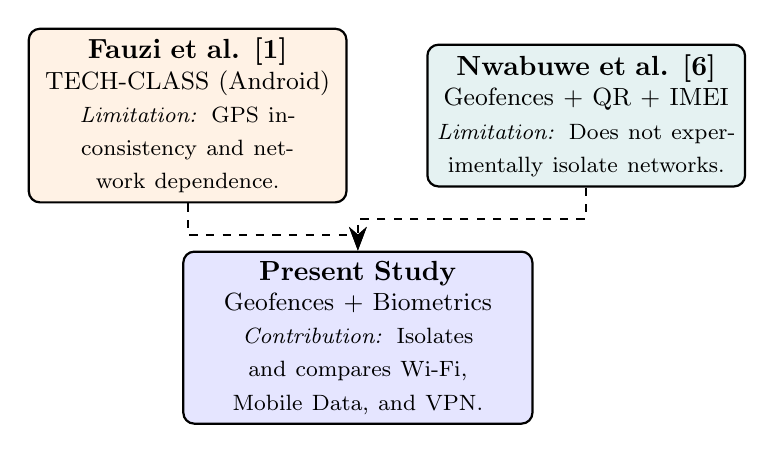
\begin{tikzpicture}[
        node distance=0.8cm and 1cm, 
        fauzi/.style={rectangle, draw=black, thick, fill=orange!10, text width=3.8cm, align=center, minimum height=1.8cm, rounded corners},
        nwabuwe/.style={rectangle, draw=black, thick, fill=teal!10, text width=3.8cm, align=center, minimum height=1.8cm, rounded corners},
        propuesta/.style={rectangle, draw=black, thick, fill=blue!10, text width=4.2cm, align=center, minimum height=1.8cm, rounded corners},
        arrow/.style={-{Stealth[length=3mm]}, thick, dashed}
    ]
    
    \node (fauzi_node) [fauzi] {\textbf{Fauzi et al. [1]}\\ \small TECH-CLASS (Android)\\ \footnotesize \textit{Limitation:} GPS inconsistency and network dependence.};
    
    \node (nwabuwe_node) [nwabuwe, right=of fauzi_node] {\textbf{Nwabuwe et al. [6]}\\ \small Geofences + QR + IMEI\\ \footnotesize \textit{Limitation:} Does not experimentally isolate networks.};
    
    \node (propuesta_node) [propuesta, below=0.8cm of nwabuwe_node, xshift=-2.9cm] {\textbf{Present Study}\\ \small Geofences + Biometrics\\ \footnotesize \textit{Contribution:} Isolates and compares Wi-Fi, Mobile Data, and VPN.};
    
    \draw [arrow] (fauzi_node.south) -- ++(0,-0.4) -| (propuesta_node.north);
    \draw [arrow] (nwabuwe_node.south) -- ++(0,-0.4) -| (propuesta_node.north);
    
    \end{tikzpicture}%
    }
    \caption{Evolution of attendance validation mechanisms and research gaps addressed by the present study.}
    \label{fig:comparacion_autores}
\end{figure}

The combination of location and biometrics has also been addressed in previous works. Alburaiki et al. \cite{alburaiki2021} integrated facial recognition and location detection using machine learning in a mobile attendance system. Likewise, Alhanaee et al. \cite{alhanaee2021} evaluated transfer learning models for facial recognition, prioritizing identification accuracy and training time. These studies support the use of biometrics as a complementary mechanism to reduce spoofing; however, they do not analyze how network conditions can affect coordinate acquisition or the final decision of a geofence. Smart Assistance retains facial validation, but the present study limits its analysis to the geolocation layer.

From a methodological perspective, Shevchenko and Reips \cite{shevchenko2024} point out that the accuracy and sensitivity of geofences depend on factors such as the configured radius, environment, operating system, and the type of event to be detected. Complementarily, Bähr et al. \cite{bahr2020} analyzed geofences across 410 locations and documented erroneous activations, demonstrating the need to measure actual results rather than assuming every detection represents a valid presence. Kuhlmann et al. \cite{kuhlmann2021} also identified variations between devices and mobile sensor capture modes. Although their study focuses on orientation sensors, it provides an important criterion for this research: maintaining the device, browser, permissions, and geofence radius constant during testing.

The use of a VPN requires an additional distinction. Komosny \cite{komosny2023} demonstrates that location derived from an IP address can vary and be altered by VPNs or proxies, and therefore should not be interpreted as direct evidence of a person's physical location. In contrast, the W3C Geolocation API \cite{w3c2022} delivers coordinates and an accuracy value obtained by the device, subject to user authorization. Therefore, the study does not seek to verify location by IP or evaluate GPS spoofing techniques; it evaluates whether, under the same device configuration, the application maintains correct validation when alternating between Wi-Fi, mobile data, and VPN. The validation flow considered for this analysis is conceptually illustrated in Figure \ref{fig:arquitectura_redes}.

\begin{figure}[htbp]
    \centering
    \resizebox{0.85\textwidth}{!}{%
    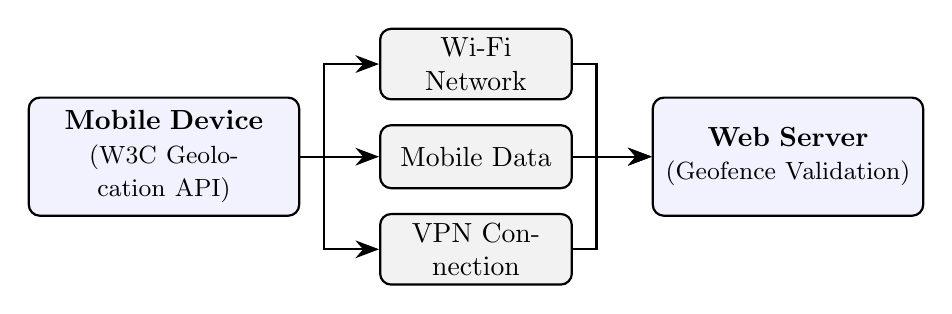
\begin{tikzpicture}[
        node distance=1.5cm and 1cm,
        box/.style={rectangle, draw=black, thick, fill=blue!5, text width=3.2cm, align=center, minimum height=1.5cm, rounded corners},
        net/.style={rectangle, draw=black, thick, fill=gray!10, text width=2.2cm, align=center, minimum height=0.8cm, rounded corners},
        arrow/.style={-{Stealth[length=3mm]}, thick}
    ]
    
    \node (device) [box] {\textbf{Mobile Device}\\ \small(W3C Geolocation API)};
    \node (datos) [net, right=of device] {Mobile Data};
    \node (wifi) [net, above=0.3cm of datos] {Wi-Fi Network};
    \node (vpn) [net, below=0.3cm of datos] {VPN Connection};
    \node (server) [box, right=of datos] {\textbf{Web Server}\\ \small(Geofence Validation)};

    \draw [arrow] (device.east) -- ++(0.3,0) |- (wifi.west);
    \draw [arrow] (device.east) -- (datos.west);
    \draw [arrow] (device.east) -- ++(0.3,0) |- (vpn.west);
    \draw [arrow] (wifi.east) -| ++(0.3,0) |- (server.west);
    \draw [arrow] (datos.east) -- (server.west);
    \draw [arrow] (vpn.east) -| ++(0.3,0) |- (server.west);
    
    \end{tikzpicture}%
    }
    \caption{Conceptual representation of the location capture and connectivity evaluation flow.}
    \label{fig:arquitectura_redes}
\end{figure}

In summary, the reviewed sources demonstrate the utility of geofences, biometrics, and additional anti-fraud mechanisms. However, as summarized in Table \ref{tab:comparacion}, they do not report a controlled comparison combining Wi-Fi, mobile data, VPN, and positions inside or outside a geofence in a distributed biometric attendance web system. The contribution of this work consists of covering this aspect through metrics of location acquisition time, reported accuracy, calculated distance to the geofence, and the acceptance or rejection result of the clock-in.

\begin{table}[H]
\centering
\caption{Comparison of previous studies on geofences and attendance control.}
\label{tab:comparacion}
\renewcommand{\arraystretch}{0.95}
\footnotesize
\begin{tabularx}{\textwidth}{@{} >{\raggedright\arraybackslash}p{2.5cm} >{\raggedright\arraybackslash}X >{\raggedright\arraybackslash}X >{\raggedright\arraybackslash}X @{}}
\toprule
\textbf{Work} & \textbf{Approach and technology} & \textbf{Metric or reported result} & \textbf{Aspect not covered compared to this study} \\
\midrule
Tamboli et al. \cite{tamboli2024} & GPS and geofencing for mobile attendance & Registration automation & Does not compare connectivity or VPN. \\

Eweoya et al. \cite{eweoya2025} & Geofence and authentication for university environment & Functional implementation & Does not measure time or accuracy under different networks. \\

Fauzi et al. \cite{fauzi2025} & Android, Geofencing API, and Firebase & SUS 95.2; 100 \% correspondence & Acknowledges connectivity dependence, without contrasting networks. \\

Nwabuwe et al. \cite{nwabuwe2023} & Dynamic QR, IMEI, and geofence & Fraud mitigation & Does not evaluate VPN or mobile data. \\

Alburaiki et al. \cite{alburaiki2021} & Facial recognition and location & Combined validation of identity and position & Does not analyze geofence stability according to network. \\

Alhanaee et al. \cite{alhanaee2021} & Facial recognition with transfer learning & Biometric accuracy and training & Does not incorporate location evaluation. \\

Shevchenko and Reips \cite{shevchenko2024} & Methodological evaluation of geofences & Influence of radius, environment, and OS & Does not study VPN in biometric attendance. \\

Bähr et al. \cite{bahr2020} & Geofences in field study & Identification of erroneous activations & Does not compare Wi-Fi and mobile data. \\

Komosny \cite{komosny2023} & IP geolocation & Geographic evidence variation due to VPN/proxy & Does not measure coordinates obtained by the device. \\

Smart Assistance (Present study) & Geofence, facial validation, and distributed architecture & Time, accuracy, distance, and acceptance/rejection & Evaluates Wi-Fi, mobile data, and VPN under controlled conditions. \\
\bottomrule
\end{tabularx}
\end{table}

\section{Solution Architecture}

Smart Assistance is used as an experimental environment to evaluate geofence validation under Wi-Fi, mobile data, and VPN connections. The application runs on Docker Swarm, where the React frontend has two replicas and the Spring Boot backend has three replicas. Swarm's native load balancing distributes requests among available instances, while PostgreSQL Neon is maintained as the single source of relational data. This configuration allows testing to be performed on a distributed architecture without duplicating attendance records.

The analyzed flow begins in the employee's browser, which requests permission to obtain the device's coordinates via the Geolocation API. The frontend transmits the location, reported accuracy, and required data to the backend via secured REST services. Subsequently, the backend validates the session using JWT, calculates the distance to the configured geofence, and determines whether the clock-in should be accepted or rejected. For each execution, the connectivity type, VPN usage, location acquisition time, accuracy, calculated distance, and validation result are recorded.

The artificial intelligence service runs in a single replica and communicates with the backend for facial biometric validation. Although this component strengthens clock-in authenticity, it does not constitute a comparison variable in the connectivity tests. Similarly, PocketBase stores the photographs associated with employees, and PostgreSQL retains attendance, auditing, and geofence configuration data.

The architecture also features an asynchronous task worker for PDF report generation and email dispatch, in addition to a Node.js gateway for Sandbox payment operations. These components are included to represent the complete solution but do not intervene in the geolocation measurement. Authentication via JWT, Google OAuth 2.0, OTP, and TOTP protects access to resources; during the experiment, the account, device, browser, permissions, and geofence radius are kept constant so that connectivity remains the main evaluated variable.

\begin{figure}[htbp]
    \centering
    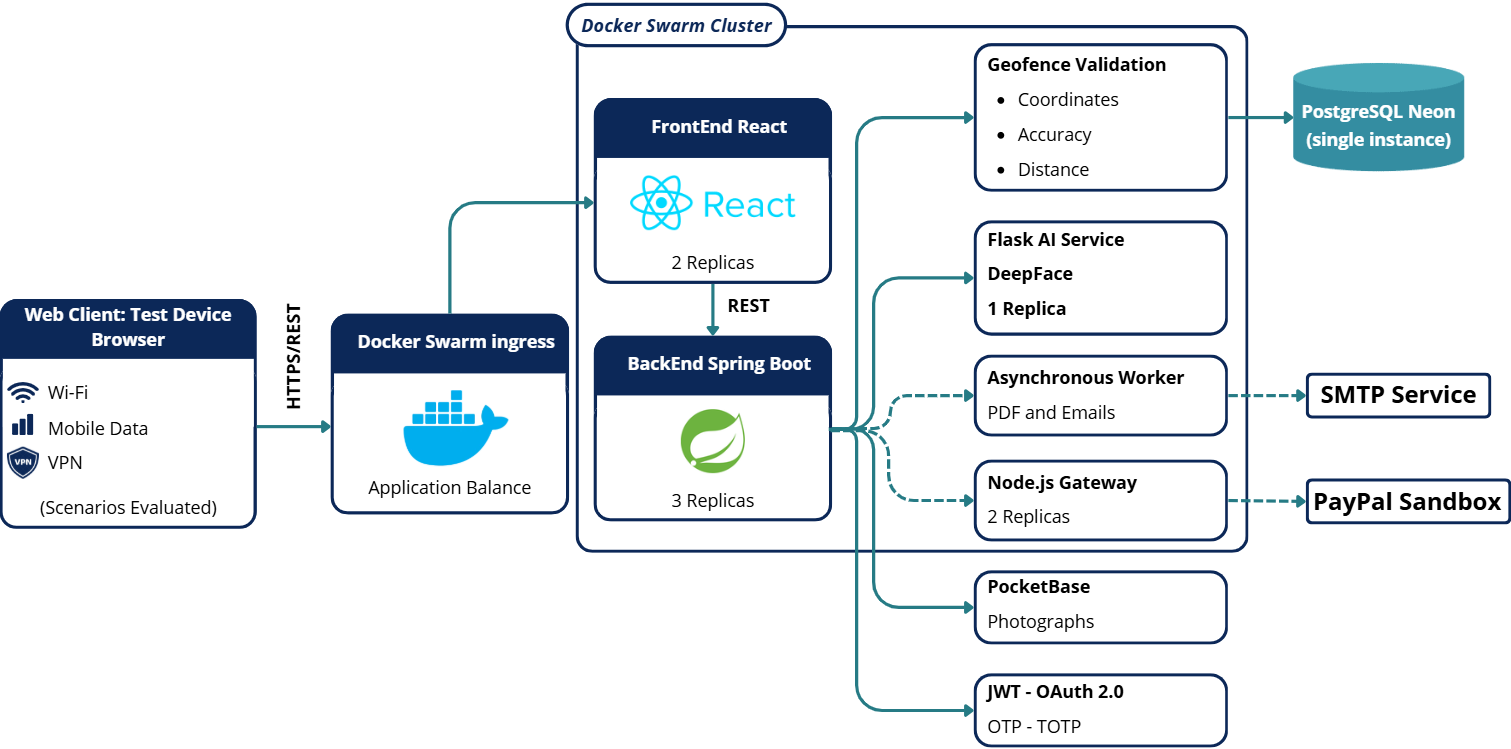
\includegraphics[scale=0.35]{images/Architecture.png}
    \caption{Architecture evaluated in the system.}
    \label{fig:architecture_jpg}
\end{figure}

\section{Methodology}
\subsection{Study Design}
A quantitative experimental study was conducted using a 2 × 2 × 2 factorial design. The purpose was to determine the effect of the connectivity type, the use of a virtual private network, and the position relative to a geofence on the behavior of Smart Assistance's georeferenced validation. The experimental unit corresponds to an individual clock-in request generated from the test device's browser.

The independent variables were: connection type, with two levels corresponding to Wi-Fi and mobile data; VPN status, with enabled and disabled levels; and physical position, classified as inside or outside the geofence. To prevent other factors from affecting the comparison, the device, browser, test account, location permissions, geofence radius, application version, and Docker Swarm cluster configuration were kept constant.

\subsection{Environment and Tools}
The tests were executed on Smart Assistance deployed in Docker Swarm. The React frontend was maintained with two replicas and the Spring Boot backend with three replicas; the PostgreSQL Neon database was used as the single source of persistence. Coordinate acquisition was performed using the Geolocation API available in the browser, while the backend applied the distance rule relative to the geofence to accept or reject the clock-in.

The client environment consisted of the Acer Aspire A515-57 device, Windows 11 Pro operating system, and Chrome browser. Cloudflare 2026.4.1350.0 was used for the VPN tests. The mobile data condition was implemented by connecting the laptop to the phone's hotspot. Browser development tools, application logs, and information stored in the database were used to capture times, coordinates, reported accuracy, and the result of each request.

\subsection{Evaluated Scenarios}
Eight scenarios, generated by the combination of the three independent variables, were evaluated as detailed in Table \ref{tab:escenarios_prueba}. The VPN was not considered an additional connection type, but rather a condition applied over Wi-Fi or mobile data.

\begin{table}[htbp]
\centering
\caption{Test scenarios configured for the evaluation.}
\label{tab:escenarios_prueba}
\renewcommand{\arraystretch}{1.2} 
\begin{tabular}{@{}clll@{}}
\toprule
\textbf{Scenario} & \textbf{Connection} & \textbf{VPN} & \textbf{Expected Position} \\
\midrule
E1 & Wi-Fi & Disabled & Inside the geofence \\
E2 & Mobile data & Disabled & Inside the geofence \\
E3 & Wi-Fi & Enabled    & Inside the geofence \\
E4 & Mobile data & Enabled    & Inside the geofence \\
E5 & Wi-Fi & Disabled & Outside the geofence \\
E6 & Mobile data & Disabled & Outside the geofence \\
E7 & Wi-Fi & Enabled    & Outside the geofence \\
E8 & Mobile data & Enabled    & Outside the geofence \\
\bottomrule
\end{tabular}
\end{table}

Two physical reference points were defined: one located within the configured radius and another outside said limit. Both points must be kept sufficiently far from the edge of the geofence to prevent a normal coordinate variation from altering the expected classification. The radius used was 10 meters; the approximate distance of the internal and external points from the center was 1 and 20 meters, respectively.

\subsection{Variables and Metrics}
The dependent variables were the location acquisition time, the accuracy reported by the browser, the calculated distance relative to the geofence, and the validation result. The reported accuracy corresponds to the \textit{accuracy} attribute of the Geolocation API, expressed in meters; therefore, it represents the estimation delivered by the device and not an absolute proof of geographic exactness.

The dependent variables were the location acquisition time, the accuracy reported by the browser, the calculated distance relative to the geofence, and the validation result, whose definitions and measurement units are summarized in Table \ref{tab:metricas_evaluacion}. The reported accuracy corresponds to the \textit{accuracy} attribute of the Geolocation API, expressed in meters; therefore, it represents the estimation delivered by the device and not an absolute proof of geographic exactness.

\begin{table}[H] % Remember to use [H] if you need it not to float to another page
\centering
\caption{Metrics and dependent variables evaluated in the study.}
\label{tab:metricas_evaluacion}
\renewcommand{\arraystretch}{1.1} % Adds a bit of vertical space for better readability
\small
% The tabularx X configuration in the central column allows the description to automatically adjust to the page width.
\begin{tabularx}{\textwidth}{@{} >{\raggedright\arraybackslash}p{2.7cm} >{\raggedright\arraybackslash}X >{\raggedright\arraybackslash}p{2.5cm} @{}}
\toprule
\textbf{Metric} & \textbf{Description} & \textbf{Unit or result} \\
\midrule
Location acquisition time & Interval between requesting the location and receiving the coordinates in the browser & Milliseconds or seconds \\
Reported accuracy & \textit{Accuracy} value reported by the Geolocation API & Meters \\
Distance to the geofence & Distance calculated by the application between the received location and the configured point & Meters \\
Response time & Interval between sending the clock-in and receiving the backend response & Milliseconds or seconds \\
Validation result & Decision issued by the backend & Accepted, rejected, or error \\
Correct validation rate & Coincidence between the obtained result and the expected physical position & Percentage (\%) \\
Failure rate & Requests without location, expired, or with communication error & Percentage (\%) \\
\bottomrule
\end{tabularx}
\end{table}

For an internal position, an accepted response was recorded as a correct validation. For an external position, a rejected response was considered correct. An external acceptance was classified as a false positive, and an internal rejection as a false negative.

\subsection{Data Used}
An external biometric dataset was not used for the analysis. The study data were generated during the execution of the tests and corresponded to technical geolocation and validation records. A previously authenticated test account was used, and photographs or personal data were not part of the analyzed metrics.

Each record stored: test identifier, date and time, scenario, connection type, VPN status, expected position, latitude, longitude, reported accuracy, calculated distance, acquisition time, response time, and final result. The exact coordinates and data that allow identifying a person must not be published in the article.

\subsection{Execution Procedure}
Initially, it was verified that the Docker Swarm services and the configured replicas were active. Subsequently, a session was started with the same test account, location permissions were granted to the browser, and it was verified that the geofence maintained the same center and radius throughout the experimentation.

For each scenario, the corresponding connection was configured, and the VPN was enabled or disabled. Next, the device was positioned at the defined internal or external point, and the clock-in request was executed. The metrics obtained in the browser, in the backend response, and in the system logs were recorded. Before the next execution, the connectivity and VPN status were checked again.

Each scenario was repeated 20 times, for a total of 160 clock-in requests. The order of the scenarios was alternated to reduce the effect of temporal changes in the signal, network availability, or location accuracy.

\subsection{Data Processing and Analysis}
At the end of each execution, the data were recorded in a CSV spreadsheet format, using a unique identifier for each test. The records were classified according to the evaluated scenario, connection type, VPN status, and expected position relative to the geofence. Cases in which no coordinates were obtained, a timeout occurred, or a server error was received were not removed; they were kept and classified as execution failures.

For each scenario, descriptive measures of central tendency and dispersion were calculated for the location acquisition time, reported accuracy, calculated distance, and response time. The correct validation rate was obtained by dividing the number of clock-ins whose result matched the expected position for each scenario. Similarly, the failure rate was calculated from the requests that did not complete the location acquisition or validation.

Finally, the data were compared by grouping the executions by connection type and VPN status. This procedure allowed identifying differences in the geofence behavior without modifying the other conditions of the experimental environment. The values, comparative tables, charts, and evidence obtained from this analysis are presented in the results section.

\section{Results}
The experimental tests generated a total of 160 georeferenced clock-in records, corresponding to 20 repetitions for each of the eight proposed scenarios. The location acquisition time on the client, the validation response time by the backend, the calculated distance, and the final status of the request were extracted. Table \ref{tab:resultados_generales} presents the average values obtained.

\begin{table}[htbp]
\centering
\caption{Average results grouped by connectivity scenario ($N=20$ per scenario).}
\label{tab:resultados_generales}
\renewcommand{\arraystretch}{1.2}
\resizebox{\textwidth}{!}{
\begin{tabular}{@{}lcccccc@{}}
\toprule
\textbf{Scen.} & \textbf{Network / VPN} & \textbf{Position} & \textbf{Acquisition (ms)} & \textbf{Response (ms)} & \textbf{Distance (m)} & \textbf{Success Rate} \\
\midrule
E1 & Wi-Fi / No & Inside & 1144.7 & 344.3 & 5.0 & 100\,\% \\
E2 & Data / No & Inside & 917.5 & 1799.9 & 1.6 & 100\,\% \\
E3 & Wi-Fi / Yes & Inside & 357.6 & 1619.2 & 3.4 & 100\,\% \\
E4 & Data / Yes & Inside & 541.7 & 6105.2 & 2.7 & 95\,\% \\
E5 & Wi-Fi / No & Outside & 3.6 & 541.0 & 24.8 & 100\,\% \\
E6 & Data / No & Outside & 3.0 & 1236.2 & 20.8 & 100\,\% \\
E7 & Wi-Fi / Yes & Outside & 3.2 & 3532.6 & 29.2 & 100\,\% \\
E8 & Data / Yes & Outside & 3.0 & 3854.8 & 28.2 & 100\,\% \\
\bottomrule
\end{tabular}%
}
\end{table}
\subsection{Validation Rate and Accuracy}
The system demonstrated high reliability in decision-making, achieving an overall correct validation rate of 99.37\,\%. Out of the 160 clock-ins, 159 were correctly classified according to the actual physical position of the device. The only inconsistency occurred in scenario E4 (Mobile data with VPN, inside the geofence), where a false negative was recorded. In this execution, the normal variation of the network coordinates placed the device 14.38 meters from the center, exceeding the 10-meter limit and causing a justified rejection by the backend, despite the user being physically inside the area.

Regarding the accuracy delivered by the Geolocation API (\textit{accuracy}), the values consistently fluctuated between 99 and 114 meters, which is characteristic of estimates based on cell towers and wireless networks in environments where the direct satellite signal is mitigated. 

It should be noted that for scenarios E5 to E8, the location acquisition time in the browser dropped drastically to an average of $\sim$3 ms. This demonstrates the intervention of the Google Chrome browser's optimization and caching mechanisms, which reuse recent coordinates if the device does not report a significant change in movement, accelerating the process on the client.

\subsection{Impact of Connectivity on Response Time}
The analysis of the server's response time revealed significant variations attributable exclusively to the network layer. As illustrated in Figure \ref{fig:tiempo_respuesta}, connections via Wi-Fi without VPN presented the most agile performance, with an average of 443 ms of total latency. When switching to mobile data networks without VPN, the response time rose to an average of 1518 ms.

The introduction of the virtual private network (VPN) severely affected communications performance. For Wi-Fi connections, the VPN multiplied the latency by six, reaching 2576 ms. The impact was even more critical in mobile data networks, where the encryption tunnel and the geographic redirection inherent to the VPN raised the response time to an average of 4980 ms (with peaks of up to 6105 ms recorded in scenario E4).

\begin{figure}[htbp]
    \centering
    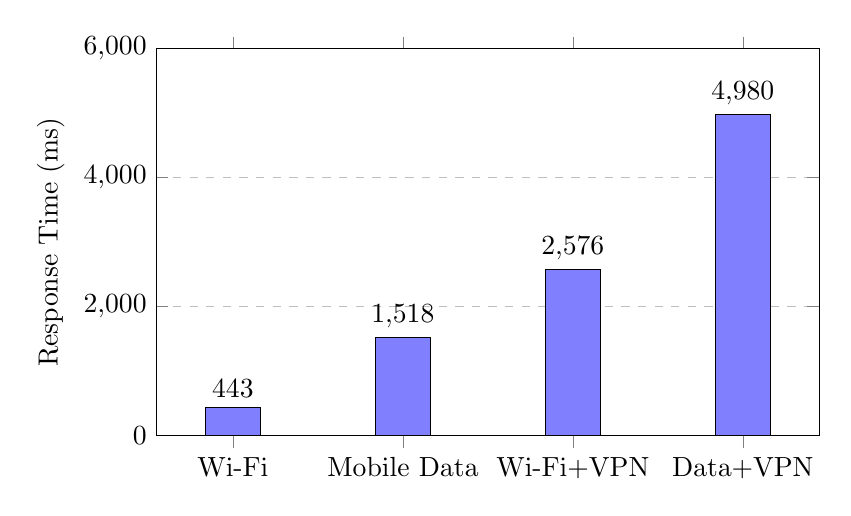
\begin{tikzpicture}
        \begin{axis}[
            ybar,
            bar width=20pt,
            width=10cm,
            height=6.5cm,
            enlarge x limits=0.15,
            ylabel={Response Time (ms)},
            symbolic x coords={Wi-Fi, Mobile Data, Wi-Fi+VPN, Data+VPN},
            xtick=data,
            nodes near coords,
            nodes near coords align={vertical},
            ymin=0, ymax=6000,
            ymajorgrids=true,
            grid style=dashed,
        ]
        
        \addplot[fill=blue!50] coordinates {
            (Wi-Fi, 443)          
            (Mobile Data, 1518) 
            (Wi-Fi+VPN, 2576)     
            (Data+VPN, 4980)     
        };
        \end{axis}
    \end{tikzpicture}
    \caption{Impact of the network type and VPN use on the average web server response time.}
    \label{fig:tiempo_respuesta}
\end{figure}

\subsection{Data Availability and Evidence}
To ensure the transparency and reproducibility of this research, the raw records obtained during the experimental phase have been published in an open-access repository. The original dataset (in CSV format) contains the timestamps, masked coordinates, reported accuracy, and exact latency times for each of the 160 requests generated across the eight scenarios. 

The results file and the execution evidence can be consulted and downloaded for their respective technical audit through the following link: 
\url{https://github.com/EdithChuico/P3Pract_ChuicoEdith.git}

\section{Discussion}

The present study answered the research question regarding the effect of connectivity and the use of a VPN on a geofence-based biometric attendance system. The data obtained mean that, although the Geolocation API is highly resilient to network manipulation (achieving 99.37\,\% accuracy in spatial classification), the connectivity layer does exert a direct and measurable impact on latency and the variability of the reported coordinates. This demonstrates that presence validation does not depend solely on physical position, but on how the device resolves said position through the available communication channels.

The observed differences, particularly the false negative in the scenario with mobile data and VPN, occurred due to the way modern devices calculate location. When routing traffic through an encrypted tunnel over a cellular network, Assisted GPS (A-GPS) triangulation loses efficiency. The device is forced to estimate its location based on distant cell towers without the rapid support of local location servers, which increased the margin of error to 14.38 meters. Unlike what was stated by Fauzi et al. \cite{fauzi2025}, who attributed the failures of their system exclusively to the inconsistency of indoor GPS hardware, this research evidences that logical network alteration generates geographic deviations of equal magnitude.

On the other hand, the findings coincide with and extend the assertions of Komosny \cite{komosny2023}. Since the VPN masked the client's IP address, a traditional system would have validated the attendance in a different country or rejected the request by default. The main advantage of the Smart Assistance proposal lies in its capacity to isolate the network layer from the sensor layer: by delegating coordinate acquisition to the browser and not to the IP, the system successfully mitigated the geographic spoofing attempt. However, as an important limitation, this design introduces an absolute dependence on browser caching; as observed, response times of $\sim$3 ms indicate that Chrome aggressively reuses previous coordinates to save energy, just as Shevchenko and Reips \cite{shevchenko2024} methodologically warn. This could allow a user to clock in just outside the edge of the geofence if their device reuses a coordinate saved seconds earlier while still inside.

Furthermore, the excessive latency times (exceeding 5 seconds under VPN and mobile data) reveal an aspect that Eweoya et al. \cite{eweoya2025} and Nwabuwe et al. \cite{nwabuwe2023} did not consider in their functional metrics. An advantage of the evaluated distributed architecture is its robustness against these delays, but the limitation lies in the user experience, as prolonged times can cause manual process cancellation or timeout errors during simultaneous biometric validation.

Regarding application contexts, the results demonstrate that this solution is highly viable for attendance control in higher education academic venues, decentralized campuses, and the management of operative personnel in fieldwork, where the installation of physical biometric equipment is economically unfeasible.

Finally, there are threats that affect the generalization and validity of the study. The experimental unit was limited to a single device model (Acer Aspire A515-57) running Windows 11 and Chrome, using \textit{tethering} to simulate mobile data. Consequently, sensor performance, operating system permissions, and battery saving policies could vary significantly when replicating the experiment on native Android or iOS hardware. Likewise, the evaluated physical environment was static and of reduced dimensions; future tests should incorporate broader geofences, real-time movement, and malicious coordinate interception to strengthen the external validity of the results.

\section{Conclusions}

The present study answered the research question regarding the effect of connectivity and VPN use in a biometric attendance system, determining that the network layer directly influences latency and the stability of spatial measurements. The main finding indicates that the combination of mobile data networks with VPN tunnels degrades the efficacy of Assisted GPS (A-GPS) triangulation, inducing anomalous variations of up to 14.38 meters that can trigger false negatives, and multiplying the server's response time to over 5 seconds.  

The fundamental contribution of this research consists of isolating and experimentally proving that geographic deviations do not stem exclusively from GPS hardware limitations, but from the logical manipulation of the network. Likewise, the study demonstrated that basing the spatial decision on the Geolocation API, rather than the IP address, successfully mitigates geographic spoofing attempts, achieving 99.37\,\% accuracy in clock-in classification. 

These results were obtained under controlled conditions, employing a static client environment (Acer Aspire A515-57 device with Windows 11 and Chrome browser), against a 10-meter radius geofence and simulating mobile data via \textit{tethering}. Consequently, the main limitation of the study lies in the use of a single browser-based execution environment, whose aggressive caching policies (with acquisition times under 5 ms) condition the behavior of the readings.  

Derived from the tests, it is recommended that attendance applications impose strict age restrictions on sensor readings, to prevent the system from processing clock-ins at the geofence boundaries using cached coordinates. Furthermore, it is suggested to implement asynchronous validation mechanisms in the backend to prevent interruptions or timeouts in the face of high latencies.  

As possible lines of future work, it is proposed to extend this experimental design to native mobile applications (Android and iOS) to evaluate the direct management of permissions and sensors by the operating system. Finally, it is proposed to broaden the evaluation by incorporating dynamic geofences with users in continuous movement to strengthen the external validity of the architecture.

% ---- Bibliography ----
%
\begin{thebibliography}{14}
\small

\bibitem{fauzi2025}
Fauzi, A. A. C., Ruzana, N., Mat, A., Ashafiqa, N., \& Fauzi, A. (2025). TECH-CLASS: A geofencing-driven attendance management system for higher education. \textit{Journal of Mathematics and Computing Science}, 11(2), 61--70. \url{https://doi.org/10.24191/jmcs.v11i2.9707}

\bibitem{w3c2022}
World Wide Web Consortium (W3C). (2022). \textit{Geolocation. W3C Recommendation}. \url{https://www.w3.org/TR/geolocation/}

\bibitem{casey2020}
Casey, E., Jaquet-Chiffelle, D.-O., Spichiger, H., Ryser, E., \& Souvignet, E. (2020). Structuring the evaluation of location-related mobile device evidence. \textit{Forensic Science International: Digital Investigation}, 32, 300928. \url{https://doi.org/10.1016/j.fsidi.2020.300928}

\bibitem{tamboli2024}
Tamboli, M., Katore, G., Patale, S., \& Philips, N. J. (2024). Attendance management system using geofencing technology. In \textit{2024 First International Conference on Pioneering Developments in Computer Science \& Digital Technologies (IC2SDT)}, pp. 137--141. \url{https://doi.org/10.1109/IC2SDT62152.2024.10696345}

\bibitem{eweoya2025}
Eweoya, I., Adeniyi, O. J., Awoniyi, A. O., Mgbeahuruike, E., Adewuyi, J. O., Adigun, T. O., \& Mensah, Y. A. (2025). Design and implementation of a university attendance management system using geo-fencing. \textit{Asian Journal of Computer Science and Technology}, 14(1), 28--46. \url{https://doi.org/10.70112/ajcst-2025.14.1.4323}



\bibitem{nwabuwe2023}
Nwabuwe, A., Sanghera, B., Alade, T., \& Olajide, F. (2023). Fraud mitigation in attendance monitoring systems using dynamic QR code, geofencing and IMEI technologies. \textit{International Journal of Advanced Computer Science and Applications}, 14(4), 938--945. \url{https://doi.org/10.14569/IJACSA.2023.01404104}

\bibitem{alburaiki2021}
Alburaiki, M. S. M., Johar, G. M., Helmi, R. A. A., \& Alkawaz, M. H. (2021). Mobile based attendance system: Face recognition and location detection using machine learning. In \textit{2021 12th Control and System Graduate Research Colloquium}, pp. 177--182. \url{https://doi.org/10.1109/ICSGRC53186.2021.9515221}

\bibitem{alhanaee2021}
Alhanaee, K., Alhammadi, M., Almenhali, N., \& Shatnawi, M. (2021). Face recognition smart attendance system using deep transfer learning. \textit{Procedia Computer Science}, 192, 4093--4102. \url{https://doi.org/10.1016/j.procs.2021.09.184}

\bibitem{shevchenko2024}
Shevchenko, Y., \& Reips, U. D. (2024). Geofencing in location-based behavioral research: Methodology, challenges, and implementation. \textit{Behavior Research Methods}, 56, 6411--6439. \url{https://doi.org/10.3758/s13428-023-02213-2}

\bibitem{bahr2020}
Bähr, S., Haas, G. C., Kreuter, F., Trappmann, M., \& Keusch, F. (2020). Using geofences to collect survey data: Lessons learned from the IAB-SMART study. \textit{Survey Methods: Insights from the Field}, 1--12. \url{https://doi.org/10.13094/SMIF-2020-00023}

\bibitem{kuhlmann2021}
Kuhlmann, T., Garaizar, P., \& Reips, U. D. (2021). Smartphone sensor accuracy varies from device to device in mobile research: The case of spatial orientation. \textit{Behavior Research Methods}, 53(1), 22--33. \url{https://doi.org/10.3758/s13428-020-01404-5}

\bibitem{komosny2023}
Komosny, D. (2023). Evidential value of country location evidence obtained from IP address geolocation. \textit{PeerJ Computer Science}, 9, e1305. \url{https://doi.org/10.7717/peerj-cs.1305}


\end{thebibliography}
\end{document}

```